\chapter{Operações Algébricas}

 Expressões algébricas são expressões matemáticas que envolvem números, letras e operações.

 Como por exemplo:

 \begin{eqnarray*}
  2x=4,\\
  x^2+1=0,\\
  x(x+3)=5,\\
  2x+3y=17,\\
  x^2 + 2y + 3z -4= 52, \\
  \frac{14x + 8y}{2x}= 3, \\
  \frac{2}{5}x^3 + 3\sqrt{x^4}= 67, \\
  5x(x+3)-4x(2-x)=7.
 \end{eqnarray*}

 Nestas expressões as letras que aparecem são chamadas de \textbf{variáveis}, e os números que aparecem multiplicando uma letra são chamados de \textbf{coeficientes}.

 As expressões algébricas são utilizadas dentre outras coisas, para descrever uma situação problema na qual não conhecemos todos os valores envolvidos, representar uma fórmula, ou expressar uma equação. Devido a sua importância nas exatas precisamos compreender como se comportam as operações presentes nas expressões algébricas, em outras palavras, como fazer contas com letras.

 \vskip0.3cm

 \textbf{Adição e subtração}

 Podemos somar somente letras iguais e com mesmo expoente. Como por exemplo:

 \begin{itemize}
  \item $2x + x= (2+1)x= 3x$
  \item $x^2 - 3x^2= (1-3)x^2= -2x^2$
  \item $2x + y + 5x^2 + 7y - 3x= 5x^2 + (2-3)x + (1+7)y= 5x^2 - 1x + 8y$
  \item $3(x+ 4y-2)= 3x + 3.4y - 3.2= 3x + 12y - 6$
 \end{itemize}

  \vskip0.3cm

 \textbf{Multiplicação}

 Na multiplicação devemos sempre multiplicar coeficiente por coeficiente e letra por letra. Sendo que no caso das letras serem iguais, devemos manter a letra e somar seus expoentes, e no caso das letras serem diferentes apenas fazemos a associação das duas letras. Como mostram os seguintes exemplos:

  \begin{itemize}
   \item $x \cdot x = x^{1+1}= x^2$
   \item $x \cdot x^2= x^{1+2}= x^3$
   \item $x \cdot 2y= (1 \cdot 2)xy= 2xy$
   \item $3x \cdot 2x^2y= (3 \cdot 2)x^{1+2}y= 6x^3y$
   \item $4x^4 \cdot \frac{1}{2}x^{-2}= (4 \cdot \frac{1}{2})x^{4-2}= 2x^2$
   \item $(x - 1) \cdot (x - 2)= x(x-2) - 1(x-2)= x^2 -2x -x +2= x^2 - 3x + 2$
  \end{itemize}

  \vskip0.3cm

   \textbf{Divisão}

   Na divisão devemos sempre dividir coeficiente por coeficiente e letra por letra. Sendo que no caso das letras serem iguais, devemos manter a letra e subtrair seus expoentes, e no caso das letras serem diferentes apenas fazemos a associação das duas letras. Como mostram os seguintes exemplos:

  \begin{itemize}
   \item $x \div x= x^{1-1}= x^0= 1$
   \item $x \div x^2= x^{1-2}= x^{-1}= \frac{1}{x}$
   \item $2y \div x= 2\frac{y}{x}$
   \item $4y^3 \div 2y^2= \frac{4}{2} \cdot \frac{y^3}{y^2}= 2y^{3-2}= 2y$
   \item $\frac{x^2yz^3}{x^2y^3z^2}= x^{2-2}y^{1-3}z^{3-2}= x^0 y^{-2}z^{1}= \frac{z}{y^2}$
   \item $\frac{(x+3) \cdot (x-1)}{(x-1)\cdot (2x+3)}= \frac{x+3}{2x+3}$
  \end{itemize}

 \vskip0.3cm

  \textbf{Potenciação}

  Na potenciação devemos aplicar o expoente ao coeficiente e à incógnita, obedecendo as propriedades de potência.

    \begin{itemize}
     \item $(2x)^2= 2^2 \cdot x^2= 4x^2$
     \item $(3x^2)^3= 3^3 \cdot x^{2\cdot 3}= 27x^6$
     \item $\left(\frac{3a^2}{4}\right)^2= \frac{3^2 a^{2 \cdot 2}}{4^2}= \frac{9a^4}{16}$
    \end{itemize}

  \vskip0.3cm

  \textbf{Radiciação}

  Na radiciação devemos extrair a raiz do coeficiente e da incógnita. Observamos que extrair a raiz da incógnita é equivalente a dividir seu expoente pelo índice da raiz.
    \begin{itemize}
     \item $\sqrt{x}= x^{\frac{1}{2}}$
     \item $\sqrt{x^4}= (x^4)^{\frac{1}{2}}= x^{\frac{4}{2}}= x^2$
     \item $\sqrt[3]{8x^6}= \sqrt[3]{8} \cdot \sqrt[3]{x^6}= 2 x^{\frac{6}{3}}= 2x^2$
     \item $\sqrt{\frac{2x^2}{16}}= \frac{\sqrt{2x^2}}{\sqrt{16}}= \frac{|x|\sqrt{2}}{4}$
     \item $\sqrt{x^2}= |x|$
    \end{itemize}

 \vskip0.3cm

  \textbf{Fatoração das expressões algébricas}

 \vskip0.3cm

 A fatoração das expressões algébricas, é o que nos permite escrever a expressão como um produto de dois termos, ela é utilizada principalmente na resolução de equações, para acelerar o processo de resolução.

 Os seguintes casos de fatoração são os mais utilizados:
 \begin{itemize}
  \item Fator em comum: $x^2 + x= x(x + 1)$; $4x^2 + 6= 2(2x^2 + 3)$
  \item Agrupamento: $ax + bx + ay + by= (a+b)x+(a+b)y= (a+b)(x+y)$
  \item Trinômio quadrado perfeito (+): $(a + b)^2= a^2 + 2ab + b^2$
  \item Trinômio quadrado perfeito (-): $(a - b)^2= a^2 - 2ab + b^2$
  \item Diferença de dois quadrados: $(a + b) \cdot (a - b)= a^2 - b^2$
  \item Cubo perfeito (+): $(a+b)^3= a^3 + 3a^2b + 3ab^2 + b^3$
  \item Cubo perfeito (-): $(a-b)^3= a^3 - 3a^2b + 3ab^2 - b^3$
 \end{itemize}
 
 \newpage
 \section{Polinômios}
 
  \vskip0.3cm
 \colorbox{azul}{
 \begin{minipage}{0.9\linewidth}
 \begin{center}
  Seja $K= \R \text{ ou } \C$. Um polinômio $p$ na incógnita $x$ e com coeficientes em $K$ (simbolicamente, $p \in K[x]$) é uma expressão da forma
  \[p(x)= a_nx^n + a_{n-1}x^{n-1}+ \ldots + a_1x+ a_0= \sum_{i=0}^{n} a_ix^i ,\]
  em que os coeficientes $a_n, \ldots, a_0 \in K$, $a_n \neq 0$ e $n \in \N$. O número natural $n$ é chamado de grau do polinômio $p$, e escreve-se $gr(p)= n$. O termo $a_0$ é denominado termo constante de $p$.
 \end{center}
 \end{minipage}}
 \vskip0.3cm
 
 \begin{obs}
 Os termos polinômio e função polinomial serão considerados como sinônimos e utilizados sem distinção no decorrer deste texto.
 \end{obs}
 
 Uma função polinomial de grau $0$ é uma função constante; uma função polinomial de grau $1$ é uma função linear (ou, função afim); uma função polinomial de grau $2$ é uma função quadrática.
 
 Por simplicidade, a partir de agora iremos considerar nossos polinômios sobre $\R$, porém esta teoria pode ser estendida sem muita dificuldade para o corpo dos números complexos.
 
 \begin{defi}
 Dados um número real $k$ e o polinômio $p(x)= a_nx^n + a_{n-1}x^{n-1}+ \ldots + a_1x+ a_0$, chama-se \emph{valor numérico de $p$ em $k$} ao valor:
 \[p(k)= a_nk^n + a_{n-1}k^{n-1}+ \ldots + a_1k+ a_0 \ .\]
 \end{defi}
 
\begin{exem}
Por exemplo, se considerarmos o polinômio $p(x)= x^2 + 7x+10$, temos os seguintes valores numéricos para $p$:
\begin{eqnarray*}
p(-6)&=& (-6)^2 + 7(-6) +10= 4\\
p(-5)&=& (-5)^2 + 7(-5) +10= 0\\
p(-4)&=& (-4)^2 + 7(-4) +10= -2\\
p(-2)&=& (-2)^2 + 7(-2) +10= 0\\
p(0)&=& 0^2 + 7 \cdot 0 +10= 10\\
\end{eqnarray*}
\end{exem} 
 
 \begin{defi}
 Em particular, se $k$ é um número real tal que $p(k)= 0$, dizemos que $k$ é uma \emph{raiz} ou \emph{um zero} de $p$.
 \end{defi}
 
 \begin{exem}
 Portanto no exemplo anterior temos que $k_1= -5$ e $k_2=-2$ são raízes do polinômio $p(x)= x^2 + 7x+10$.
 \end{exem}
 
  \begin{defi}
  O polinômio nulo (ou identicamente nulo) é um polinômio da forma $p(x)= 0x^n +0x^{n-1}+ \ldots + 0x+ 0$, ou simplesmente, $p(x)= 0$. Por convenção, o grau deste polinômio será indefinido.
 \end{defi}
 
 
  \begin{teo}
  Sejam $p$ e $q$ dois polinômios em $K$, dados por:
  \[p(x)= a_nx^n + a_{n-1}x^{n-1}+ \ldots + a_1x+ a_0= \sum_{i=0}^{n} a_ix^i\]
  \[q(x)= b_nx^n + b_{n-1}x^{n-1}+ \ldots + b_1x+ b_0= \sum_{i=0}^{n} b_ix^i\]
  temos que $p=q \Leftrightarrow a_i= b_i$, para todo $i \in \{0, 1, 2, \cdots, n\}$.
 \end{teo}
 
 \begin{dem}
 Para todo $x \in \R$, temos:
 \[a_i= b_i \Leftrightarrow a_i - b_i=0 \Leftrightarrow (a_i - b_i)x^i=0 \Leftrightarrow \sum_{i=0}^{n}(a_i - b_i)x^i= 0 \Leftrightarrow\]
 \[ \sum_{i=0}^{n}a_i x^i - \sum_{i=0}^{n}b_i x^i = 0 \Leftrightarrow \sum_{i=0}^{n}a_i x^i = \sum_{i=0}^{n}b_i x^i \Leftrightarrow p(x)= q(x)\]

 \end{dem}
 
  Este Teorema mostra que, quando escrevemos um polinômio $p$ na forma 
 \[p(x)= a_nx^n + a_{n-1}x^{n-1}+ \ldots + a_1x+ a_0\]
 com $a_i \in K$, então os números $a_0, \ldots, a_n$ são determinados de modo único. 
 
 Dados dois polinômios 
 \[p(x)= a_nx^n + a_{n-1}x^{n-1}+ \ldots + a_1x+ a_0= \sum_{i=0}^{n} a_ix^i\]
  \[q(x)= b_nx^n + b_{n-1}x^{n-1}+ \ldots + b_1x+ b_0= \sum_{i=0}^{n} b_ix^i\]
  chama-se \emph{soma} de $p$ com $q$ o polinômio
  \[(p+q)(x)= (a_n+ b_n)x^n + (a_{n-1}+b_{n-1})x^{n-1}+ \ldots + (a_1+b_1)x+ (a_0+b_0)= \sum_{i=0}^{n} (a_i+b_i)x^i \ .\]
  
  \begin{teo}
  Se $p$, $q$ e $p+q$ são polinômios não nulos, então o grau do polinômio $p+q$ é menor ou igual ao maior dos números $gr(p)$ e $gr(q)$;
  \[gr(p+q) \leq \text{máx}\{gr(p), gr(q)\} \ .\]
  \end{teo}
  
  \begin{teo}
  Se $p$, $q$ e $p \cdot q$ são polinômios não nulos, então o grau do polinômio $p \cdot q$ é igual a soma dos graus de $p$ e $q$;
  \[gr(p \cdot q) = gr(p) + gr(q) \ .\]
  \end{teo}
  
  Para funções polinomiais o \emph{Teorema Fundamental da Álgebra} garante a existência de zeros.
  
  \begin{teo}[Teorema Fundamental da Álgebra]
  Seja $p \in \C[x]$ um polinômio não constante. Então existe um número complexo $z_0$ tal que $p(z_0)=0$.
  \end{teo}
  
  \begin{dem}
  A demonstração deste resultado pode ser encontrada em livros de Cálculo de uma variável complexa ou Análise Complexa como por exemplo página 119 do (SOARES, 2009).
  \end{dem}
  
  Como consequência direta do Teorema Fundamental da Álgebra temos o seguinte teorema.
  
  \begin{teo}
  Todo polinômio de grau $n \geq 1$ possui pelo menos uma raiz real ou complexa.
  \end{teo}
  
 Observe que estes resultados garantem que todo polinômio possui pelo menos uma raiz complexa, como vamos focar nossos estudos em polinômios sobre $\R$, podemos neste caso ter polinômios que não possuem raízes reais. Ainda sobre as raízes de um polinômio vale destacar o seguinte teorema.
 
 \begin{teo}
  Seja $p$ um polinômio não nulo em $K$, escrito na forma
  \[p(x)= a_nx^n + a_{n-1}x^{n-1}+ \ldots + a_1x+ a_0\]
   então $p$ tem no máximo $n$ raízes em $K$. 
 \end{teo}
 
 \begin{teo}
  Sejam $p(x)$, $g(x)$ polinômios sobre o corpo $K$, i.e., polinômios em $K[x]$, e suponhamos que $gr(g) \geq 0$. Então, existem polinômios $q(x)$ e $r(x)$ tais que
  \[p(x)= q(x)g(x) + r(x) \ , \]
  em que $gr(r) < gr (g)$. Essas condições permitem determinar os polinômio $q$ e $r$ de modo único.
 \end{teo}

 \begin{dem}
 A demonstração deste teorema pode ser encontrada na página 58 do (LANG, 1972).
 \end{dem}


 
 \begin{exem}
  Como um exemplo para a divisão de polinômios, façamos a divisão do polinômio $p_1(x)=x^3-4x^2+x+6$ pelo binômio $g_1(x)=x+1$:

 \begin{figure}[H]
 \centering
 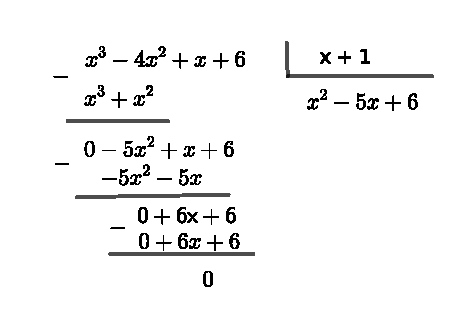
\includegraphics[width=8cm]{../Topicos/Figuras/polinomiosdivisao.pdf}
 \end{figure}
 
 note que o quociente da divisão é $q_1(x)= x^2 - 5x + 6$, e o resto desta divisão é $r(x)=0$ (zero). Como o resto é zero concluímos que $p_1(x)$ é divisível por $g_1(x)$. Portanto $p_1(x)= q_1(x)g_1(x)$, ou seja, $x^3-4x^2+x+6= (x^2-5x+6)(x+1)$.
 \end{exem}
 
 Como consequência do teorema anterior, temos o seguinte corolário, que nos garante que no exemplo anterior $-1$ é uma raiz do polinômio $p_1(x)$.
 
 \begin{cor}
 Seja $p$ um polinômio não-nulo sobre $K$. Seja $\alpha \in K$ tal que $p(\alpha)=0$. Então, existe um polinômio $q(x)$ sobre $K$ tal que 
 \[p(x)= (x - \alpha)q(x) \ .\]
 \end{cor}
 
 Como consequência deste Corolário, todo polinômio de grau $n \geq 1$ pode ser escrito como produto de $n$ fatores de grau $1$.
 
 \begin{teo}[Teorema da Decomposição]
  Todo polinômio $p(x)= a_nx^n + a_{n-1}x^{n-1}+ \ldots + a_1x+ a_0$, com $a_n \neq 0$, pode ser escrito de forma fatorada
  \[p(x)= a_n(x - r_1)(x - r_2) \ldots (x - r_n)\]
  onde $r_1, r_2, \cdots, r_n$ são as raízes do polinômio.  
 \end{teo}

